\section{Methods}
Here we describe the digital evolution system and experiment setup used to conduct this work.

% Evolution platform: Avida in MABE2
\subsection{The Avida Digital Evolution Platform}
\label{sub-evo-software}

%%%% Shorten this paragraph -- Avida was covered in the previous chapter
This work uses the Avida Digital Evolution Platform \citep{ofriaAvidaSoftwarePlatform2004a}, which was described in Chapter \ref{chap:consequences_of_plasticity}.
Here we use an early build of version 5.0 of Avida, currently under development as part of the Modular Agent Based Evolver 2 (MABE2) framework (\href{https://github.com/mercere99/MABE2}{https://github.com/mercere99/MABE2}).
%In Avida, populations of self-replicating computer programs perform tasks to compete for CPU cycles, creating an evolution testbed that can support a wide array of experimental controls. 
Avida has previously been used to study both associative learning \citep{pontesEvolutionaryOriginAssociative2020, grabowskiEarlyEvolutionMemory2010a} and historical contingency via replay experiments \citep{yedidHistoricalContingentFactors2008, covertiiiExperimentsRoleDeleterious2013}.
Fundamentally, Avida is designed to have tools necessary to conduct work at the scale required for analytic replay experiments. 
%provides the tools necessary for conducting analytic replay experiments, while its digital nature makes the scale of this work feasible. %while its digital nature keeps experiment times manageable.
%While Avida is more complex, and thus slower, than other digital evolution models, we argue that this is appropriate for initial measurements of potentiation dynamics.
%Future work can isolate which of these dynamics are explained with simpler systems and which require more complicated interactions.

% % General intro to what we used -> Avida overview and why we used it
% This work uses an early build of version 5.0 of the Avida Digital Evolution Platform \citep{ofriaAvidaSoftwarePlatform2004a}, currently under development as part of the Modular Agent Based Evolver 2 (MABE2) framework (\href{https://github.com/mercere99/MABE2}{https://github.com/mercere99/MABE2}).
% In Avida, populations of self-replicating computer programs perform tasks to compete for CPU cycles, creating an evolution testbed that can support a wide array of experimental controls. 
% Avida has been used for numerous studies on the evolution of complexity \citep{lenski_evolutionary_2003, zamanCoevolutionDrivesEmergence2014}, associative learning \citep{pontesEvolutionaryOriginAssociative2020, grabowskiEarlyEvolutionMemory2010a}, and historical contingency via replay experiments \citep{yedidHistoricalContingentFactors2008, covertiiiExperimentsRoleDeleterious2013}.
% Fundamentally, Avida is designed to have tools necessary to conduct work at the scale required for replay experiments. %provides the tools necessary for conducting analytic replay experiments, while its digital nature makes the scale of this work feasible. %while its digital nature keeps experiment times manageable.
% While Avida is more complex, and thus slower, than other digital evolution models, we argue that this is appropriate for initial measurements of potentiation dynamics.
% Future work can isolate which of these dynamics are explained with simpler systems and which require more complicated interactions.



% What is Avida? (currently more "what are organisms in Avida?")
Avida genomes consist of assembly-like instructions that transfer data between registers, make basic comparisons, perform mathematical operations, \textit{etc}.
We use an extended instruction set that includes extra flow control and environment-specific instructions \citep{fergusonFergusonAJReplayingEvolution2023}.
%The full set of 45 instructions is available in the supplement [CITE].

% Basic process of Avida
We used Avida populations on a 60x60 toroidal grid, resulting in a population cap of 3,600 organisms.
%When reproducing, an offspring is created (possibly with mutations) and 
Offspring are placed in a grid cell next to their parent, overwriting any existing organism in that cell; the parent organism is also reset. % (but not mutated). 
During reproduction, point mutations occur in offspring at a rate of 0.0075 per instruction, while single-instruction insertion and deletion mutations occur at a rate of 0.05 per reproduction.
%We do not directly decide which organisms reproduce; 
Organisms reproduce by %executing a certain number of instructions and then 
executing the \texttt{Repro} instruction.
To prevent organisms from immediately replicating, % instead of attempting the associative learning task, 
organisms must execute 1,500 instructions before the \texttt{Repro} instruction can be activated.  
%Our influence on selection takes the form of rewards and punishments in the environment.
%Organisms that maintain a positive reward/punishment balance are able to execute more instructions, on average, and thus are more likely to successfully reproduce.


% MABE info?

\subsubsection{Associative learning}
\label{subsub-environment}
% Brief overview of the environment
%Since selection pressures in Avida come from the rewards and punishments in the environment, we must decide how that environment functions, which behaviors are rewarded, and which behaviors are punished.%, and how large these rewards and punishments are.
%For this work, 
%We created an Avida environment to test the evolution of associative learning, heavily inspired by the Avida path following environment % used in previous Avida experiments 
%\citep{pontesEvolutionaryOriginAssociative2020}. %, grabowskiEarlyEvolutionMemory2010a}.
To test the evolution of associative learning, we created a simplified version of the Avida path following environment \citep{pontesEvolutionaryOriginAssociative2020}. %, further discretizing the movements along the path.
%As in the path following environment, organisms are tasked with choosing the right action given a particular nutrient cue.
%The difference is that organism evaluation no longer occurs on a two-dimensional grid. 
%At any point, 
Instead of navigating 2D space, an organism exists in one of four states: \textit{forward}, \textit{left}, \textit{right}, or the error state, \textit{backward}.
%At any point, an organism is guaranteed to be in one of of four states: \textit{forward}, \textit{left}, \textit{right}, or \textit{backward}. 
%Each state is named for the action an organism must take to obtain an associated nutrient. % and requires the organism to execute a different instruction (with the same name as the state).%, and a nutrient cue is associated with each state. 
%By removing the dependence on a two-dimensional grid, this new environment is faster to execute and allows for randomly-generated states with no fear of paths crossing over themselves. 
%
% Details as to how the organism receives information and what it is expected to do with it
Organisms are given a \texttt{Sense} instruction, which will give them the nutrient cue of their current state. 
Using this nutrient cue, organisms need to execute the appropriate instruction (one per state) to progress along the path.
The \textit{forward} and \textit{backward} states have fixed cues (0 and -1, respectively), while, at birth, each organism is assigned random cue values for \textit{left} and \textit{right} in the range of [1, $10^{6}$]. %that persist for the organism's lifetime.
Organisms can genetically encode \textit{forward} and \textit{backward}, but must learn \textit{left} or \textit{right} in their lifetime to perfectly solve the task.
Each path begins with one of four preset starting state sequences, chosen randomly for each organism at birth, followed by additional random states. % if the organism navigated through the entire preset path. 
The four preset paths are the ``one-fixed turn'' paths from \citep{pontesEvolutionaryOriginAssociative2020}, where organisms are guaranteed to encounter a \textit{left} state before a \textit{right}.

If the organism is not in an error state and executes the appropriate instruction, they are rewarded and move to the next state. 
If an organism executes the wrong instruction (e.g., the \texttt{Left} instruction in the \textit{right} state), it is penalized and placed in the error state. 
%While in the error state, the organism will be penalized for executing the other three state-associated instructions, but upon executing the \texttt{Backward} instruction it will be placed in the previous state and allowed to try again. 
While in the error state, the organism must execute the \texttt{Backward} instruction to return to the previous state and be allowed to try again; it will be penalized for any other action. 
%This means that ``resetting'' after a bad movement is much easier than in the original path following environment. 
A cooldown is applied, however, such that executing the \texttt{Backward} instruction causes the organism to wait for the equivalent of 10 additional instruction executions.
%This cooldown allows for a much simpler mechanism of self-resetting while not significantly altering the dynamics of different strategies.
Organisms are scored based on the number of valid states they successfully traversed minus the number of incorrect moves made, with a maximum score of 300. 
Fitness is calculated as $1.25^{score}$, so each additional correct movement grants a 25\% boost in fitness regardless of the total number of correct movements.


% % Why is this associative learning
% Of the four states, \textit{forward} and \textit{backward} have set nutrient cues. 
% For every organism, \textit{forward} has a cue of 0 and \textit{backward} has a cue of -1. 
% The other two states have random cues. 
% When an organism is born, its \textit{left} and \textit{right} cues are randomized to integers in $[1,10^{6}]$.
% These cues are set for the organism's lifetime.
% Therefore, while \textit{forward} and \textit{backward} decisions can be genetically encoded, \textit{left} and \textit{right} require memory to associate the random cues to their appropriate instructions. 

% What behaviors can crop up, and how do we identify them?
In this environment, optimal behavior requires associative learning in the form of imprinting. 
Since the paths are guaranteed to have a \textit{left} state before a \textit{right} state, the optimal behavior is to find and store the first positive cue value as the \textit{left} cue.
Combined with genetically-encoded \textit{forward} and \textit{backward} logic, storing and using the \textit{left} cue is enough for organisms to identify the \textit{right} cue through a process of elimination. %indefinitely pass through states without making any errors. 
%This is easier than the trial and error approach that would be needed if there were no guarantees about the starting cue, but it still requires organisms to associate at least one random cue with a state.
Other possible behaviors involve error correction (assuming all turns are one direction, then correcting when wrong), bet-hedged learning (assuming more about the paths, e.g., that there are no instances of two lefts in a row), and various mixed strategies. 

% Classification of replicates
%We then classified the dominant genotype of each replicate. 
%To sample how the genotype handles variation in the environment, we ran each genotype in 100 trials. 
%This guarantees the genotype will be tested in each of the four path starts and with a variety of random cue values. 
To categorize the behavior of a genotype, we evaluate it in 100 trials to ensure we observe how it performs in all four environments with different random cues.
We then classify each of the 100 trials.
Trials are classified as learning if the organism correctly handles greater than 90\% of the states they were in, error correction if they always successfully navigated one turn state but not the other, and ``low activity'' if they failed to successfully navigate at least 25 states.
%Trials were classified as potentially learning if they correctly handled greater than 90\% of the states they were in.
%Trials that consistently made errors in either \textit{left} or \textit{right} yet never made errors in the opposite state were classified as error correction. 
%This typically takes the form of always executing one instruction (e.g., \texttt{Left}) when in an uncertain state, and then backing up and correcting if that was the wrong instruction. 
%Finally, trials with less than 25 correct states were classified as too small to identify.
%A full breakdown of trial classification is available in the supplement [CITE]. 
%We then used the trial classifications to classify the genotype. 
To be categorized as learning or error correction, \textit{all} 100 trials of that genotype must be of that class. 
If one or more trials were low activity, the genotype was categorized as ``bet-hedged learning'' or ``bet-hedged error correction''.
If a genotype displayed at least one learning trial and at least one error correction trial, they were classified as ``mixed bet hedging''.
Finally, all remaining genotypes were categorized as ``low activity''.
%If all trials were classified as learning, the genotype was classified as learning. 
%Similarly, error correction genotypes require that all trials are classified as error correction. 
%If some trials are classified as learning and the rest are classified as too small to identify, the genotype is classified as bet-hedged learning, and the same goes for error correction and bet-hedged error correction. 
%If some trials were classified as learning and others were classified as error-correction, we classify the genotype as mixed bet-hedging. 
%Finally, if none of the other categories fit the genotype, we classify the whole genotype as too small to classify. 
This categorization system was used across all three phases of this work.

% What did we actually do?
\subsection{Experiment framework}

\begin{figure}[h!]
\begin{center}
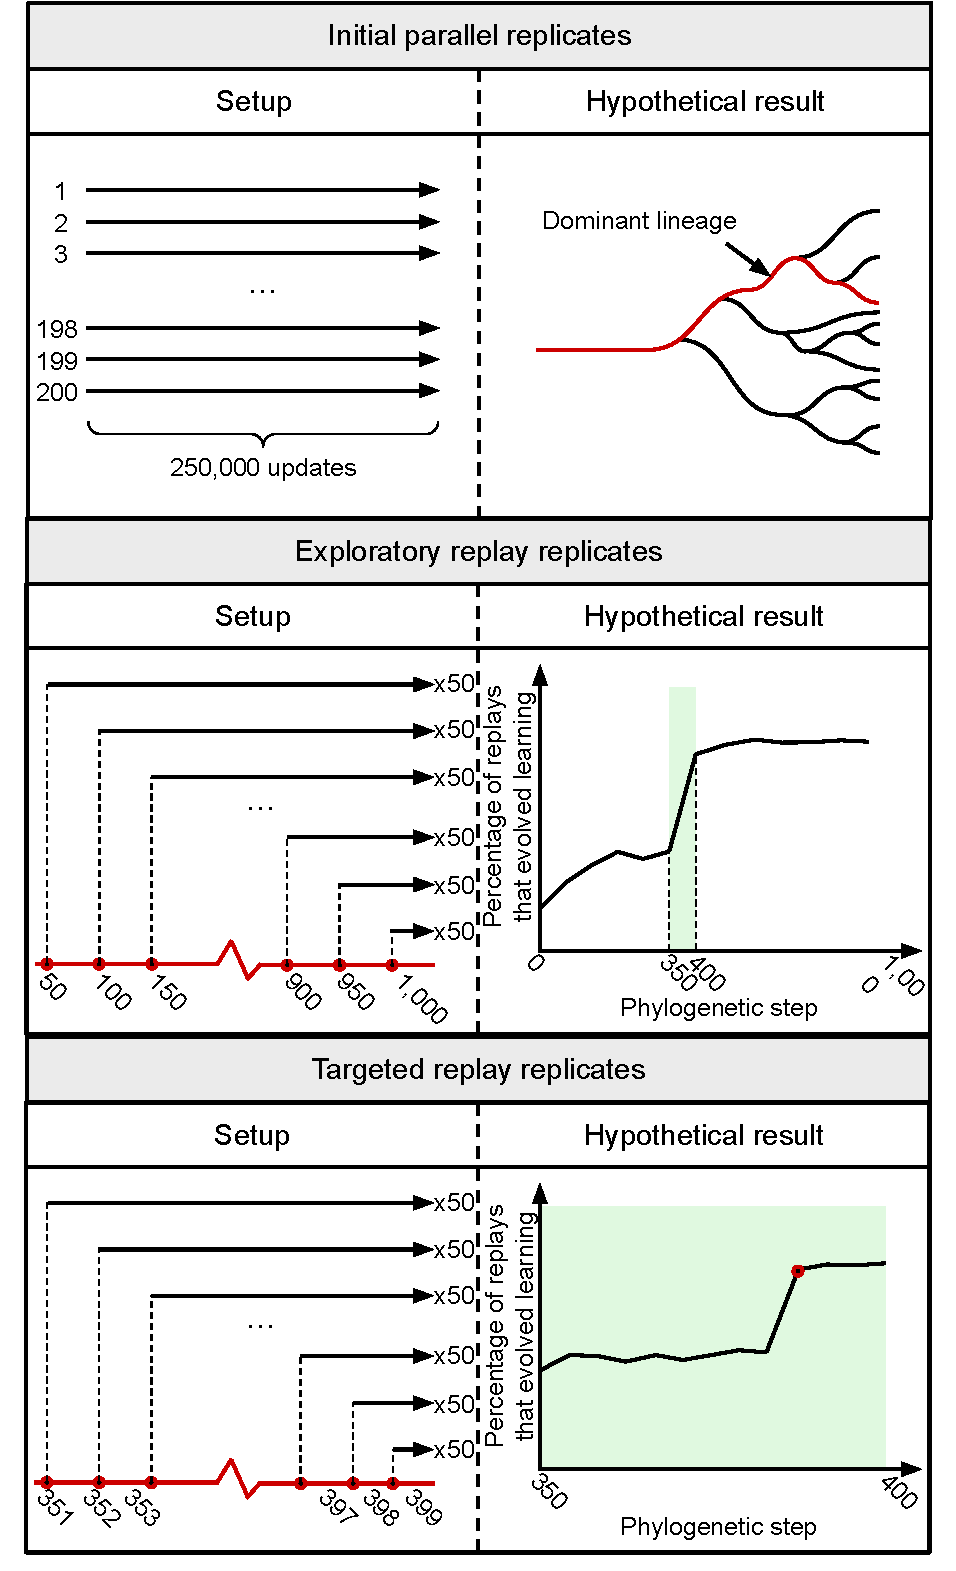
\includegraphics[width=0.65\textwidth]{03_learning_case_studies/media/conceptual_figure.pdf}
\caption{
    Illustration of the experimental design and hypothetical results.
    The top panes show the 200 initial parallel replicates seeded with the ancestral genotype and evolved for 250,000 updates.
    We extracted the lineage of the most abundant genotype in the evolved population (the dominant lineage), shown in red. 
    %When these replicates finish, we can classify each replicate and extract the dominant lineage (in red) from the phylogeny.
    Next, we conducted exploratory replays (middle panes) by launching replay replicates at regular intervals along focal lineages. 
    These exploratory replays give a coarse-grained view of how potentiation changed over a lineage. 
    We identified the window with the largest potentiation gain, shown as the shaded region.
    Finally, we ran targeted replay replicates for every step in this potentiation window. 
    %Phase 2 takes each dominant lineage from Phase 1 and launches replay experiments every 50 steps along the lineage. 
    %An example potentiation graph is shown, where a substantial increase in potentiation occurs between steps 350 and 400. 
    %We then seed \textit{additional} replay replicates for Phase 3, one for each step in the window identified in Phase 2.
    These fine-grained replay replicates show mutations that resulted in large potentiation increases (shown here with a red dot). 
}
\label{fig-conceptual}
\end{center}
\end{figure}

% Introduce three-phase design and give a brief overview of each part
To identify mutations that substantially increased the likelihood that learning evolved, we split the work into three phases (see Figure \ref{fig-conceptual} for an overview).
%
First, we seeded 200 initial parallel replicates in the associative learning environment with a default ancestor only capable of reproduction. 
Each replicate was given 250,000 updates, where one update is the time it takes for all organisms to execute 30 instructions, on average. 
% These replicates evolved for 250,000 updates, where one update is the
% and evolved them for 250,000 updates.
%For each of the 200 replicates, 
We identified the most abundant genotype in each final population to represent the replicate and classified its behavior. 
%By tracking the phylogeny in each replicate, 
We then extracted the ``dominant lineage'', stretching from the ancestor to the representative genotype. 
%(i.e., the \textit{dominant genotype} of that replicate), classified its behavior, and extracted its lineage from the ancestor. 
Each step in the lineage corresponds to a change in genotype between parent and offspring, with clonal offspring occupying the same step as their parent.
While a step is often a single mutation, it is possible that one step is composed of multiple co-occurring mutations.

To begin analyzing changes in potentiation, we ran exploratory replays replicates on four lineages capable of learning.
%Due to the computational cost of these replay experiments, we performed replays on only four learning replicates.
For each, we seeded independent replicates for every $50^{th}$ step in the lineage, up to step 1,000.
All replay replicates evolved in the same associative learning environment, and replays were given the same number of updates as had %equal to the number of updates that 
occurred after that genotype first appeared (e.g., replays for a genotype that appeared at update 150,000 would be evolved for the remaining 100,000 updates). 
Potentiation was measured as the portion of replay replicates that evolved learning. % divided by the number of replay replicates that finished. 
Because replays were seeded with a single organism, some replay populations went extinct before ever reproducing and thus were not factored in (the minimum number of finished replay replicates from a given lineage step was 38, while three case study lineages had a minimum of 48). 

While the exploratory replays provide an overview of how potentiation changed, we dug deeper by running targeted replays to further explore windows of increasing potentiation.
Specifically, we found the 50- or 100-step ``potentiation window'' that sees the largest increase in potentiation in the exploratory results, and seeded additional replays for every step in that range.
These targeted replays were conducted identically to the exploratory replays, only they did not skip steps.
Though computationally expensive, these replays illuminated the impact every genotypic change had on potentiation. 
Running 50 replay replicates per step still results in considerable noise, but we were able to identify mutations that clearly and substantially increased potentiation using these targeted replays.

We hand-analyzed algorithms in all potentiating mutations, here defined as single lineage steps that result in a potentiation increase of 25 percentage points or more.
%These potentiating mutations and other steps around them in the lineages were hand-analyzed to understand the underlying algorithm encoded in each genotype and how changes to that algorithm may have potentiated the lineage. 
Further, we assessed genotype fitness in context of their lineage to identify if potentiation mutations were beneficial, deleterious, or neutral. 
Finally, %mutation analyses were conducted to 
we characterized the local fitness landscape of each genotype (one and two mutations out), measuring the presence and fitness of nearby genotypes capable of learning. 
%All two-step mutations were analyzed for each potentiating step and the step before it, to investigate whether the potentiating step increased the presence of learning in the local landscape, increased the benefit of learning, etc. 

% We then took four lineages that exhibited learning and performed exploratory replays.
% These exploratory replays took the learning lineages and conducted a ``coarse-grained'' sampling of the lineage via analytical replay experiments. 
% We ran replay replicates for every 50 steps along the lineage, out to step 1,000. 
% This provided a window into how the likelihood of evolving learning changed over time.%, and importantly, identified any periods of substantial increases in that likelihood. 
% Finally, in we isolated these period(s) of drastic increases in likelihood and ran additional targeted replay replicates in that window (one for each step along the lineage). 
% This would then show us the impact of individual steps along the lineage, potentially highlighting single steps with massive changes in potentiation. 

% % What did our replay experiments look like?
% %\subsubsection{Analytical replay experiments}
% %After identifying the replicates that evolved learning, we can then begin to analyze their evolutionary history. 
% %We tracked phylogenetic data on all extant organisms and their ancestors, so we can trace a line of descent from the final dominant genotype to the original ancestor. 
% %After identifying the replicates that evolved learning, we then started analytical replay experiments.
% %For each learning replicate, we seeded \textit{additional} evolutionary runs along the dominant genotype's lineage. 
% %Lineages are based on genotypes, so each ``step'' corresponds to a reproduction event where one or more new mutations were introduced in the new offspring. 
% %Starting at step 50, we seeded 50 replay experiments at every $50^{\text{th}}$ step up through step 1,000. 

% %Replay replicates evolved to match the 250,000 updates of the initial replicates.
% %Replays starting from early points in the lineage thus saw more new updates than replays from points farther along the lineage. 
% %As an example, if a replay starts from step 200 and the genotype was first seen at update 100,000, we would run the replicates for step 200 for 150,000 updates. 
% %These evenly-spaced replay replicates were than manually inspected for any large jumps in potentiation. 
% %If evidence of large jumps was detected, we then seeded fine-grained replay replicates for every step between the two multiples of 50.

% % \subsubsection{Initial parallel replicates}

% % % General info, 200 reps for 250k updates starting with a default ancestor
% % We stared by founding 200 parallel replicates (see top panels of Figure \ref{fig-conceptual}). 
% % Each replicate started with one organism: the ancestor organism, which consists of 99 no-operation instructions and 1 \texttt{Repro} instruction. 
% % This organism only reproduces itself, it does not interact with the environment and thus cannot receive any rewards or punishment. 
% % Each replicate was given 250,000 updates, where one update is the time it takes for all organisms to execute 30 instructions, on average. 
% % All replicates ran in the same associative learning environment.

% % % Phylogeny tracking and isolating the final dominant genotype + lineage 
% % % CITE Emily? 
% % We tracked pruned genotypic phylogenies for these initial replicates. 
% % Digital evolution has the advantage of perfectly tracking all reproduction events and storing parent-child relationships. 
% % To reduce the storage overhead, we pruned the phylogenies to only track the extant population and any ancestors of those organisms. 
% % In the end, this gave us the lineage from the ancestral organism to any genotype in the extant population at the end of the 250,000 updates. 
% % As a representative of the final extant population, we extracted the most abundant extant genotype (i.e., the dominant genotype of that replicate) and isolated its lineage.



% \subsubsection{Exploratory replay replicates}

% After the initial parallel replicates concluded, we had a set of replicates that had evolved and maintained associative learning at the end of 250,000 updates. 
% Since we know learning evolved along each of these lineages, we are interested in how the \textit{potentiation} for learning changed along the lineages (i.e., at what points along the lineage was lineage more likely to appear than not, and where did the largest jumps in potentiation occur?).
% To investigate these changes in potentiation, we took a subset of these replicates and conducted a batch of coarse-grained replay experiments to look for large gains in potentiation while conserving computational resources.
% For a given lineage, we seeded 50 replay populations at every $50^{th}$ step along the lineage (see the middle panes of Figure \ref{fig-conceptual}.
% Regardless of the length of the lineage, we stopped at step 1,000, only continuing beyond that point if the potentiation had not approached 100\%.

% To measure potentiation at a point along the lineage, we ran the 50 replay replicates and then calculated the percentage of those replicates that evolved learning (e.g., if 30 replays out of 50 evolved learning, that point would have a potentiation of 60\%). 
% These exploratory replay replicates gave us a summary of how potentiation changed over the course of the lineage. 
% More specifically, we could look for windows containing large potentiation increases. 
% If single mutations conferred large jumps in potentiation, we would expect them to occur in windows of substantial potentiation gain.
% Since all lineages started from the same ancestor, the results from the initial parallel replicates were used for step 0 of every lineage to save computational power.

% \subsubsection{Targeted replay replicates}

% Once the exploratory replays were conducted, we had a summary of how the potentiation changed over the course of the lineage. 
% We used this exploratory replays to identify periods of drastic potentiation gain. 
% The exploratory replays occurred at every 50 steps along the lineage, so we identified the 50-step window that resulted in the greatest increase in potentiation (and for the first two lineages we took a 100-step window as to maximize our chances of finding mutations that confer large jumps in potentiation. 

% Once the target window was identified, we repeated the process of running replay experiments. 
% This time we seeded replays from every step along the lineage inside the target window. 
% While computationally expensive, this illuminates the impact every change in genotype had on potentiation. 
% While 50 replay replicates per lineage step still results in considerable variation, we were able to identify mutations that clearly and substantially increased potentiation using these targeted replays. 

% Once a potentiating step was identified, we analyzed various aspects of the genotype and the evolutionary characteristics surrounding it. 
% These potentiating steps and other steps around them in the lineages were hand-analyzed to understand the underlying algorithm encoded in each genotype and how changes to that algorithm may have potentiated the lineage. 
% Further, the genotypes were assessed in context of the lineage to identify if these potentiation events were beneficial, deleterious, or neutral in terms of fitness. 
% Finally, mutation analyses were conducted to characterize the local fitness landscape and its relationship to learning. 
% All two-step mutations were analyzed for each potentiating step and the step before it, to investigate whether the potentiating step increased the presence of learning in the local landscape, increased the benefit of learning, etc. 

% % How did we conduct our mutational analysis?
% %\subsubsection{Mutational landscape analysis}

% Not sure if we'll have real statistics, but we'll definitely have data to upload
\subsection{Data and software availability}

Both the data and the software used to conduct this work are available in the supplemental material \citep{fergusonFergusonAJReplayingEvolution2023}.
Analyses were conducted in the R statistical computing language \citep{r_core_team_r_v4} using the \textit{dplyr} package to summarize data \citep{wickhamDplyrGrammarData2022}.
Data was visualized using the \textit{ggplot2} and \textit{cowplot} packages \citep{R-ggplot2, R-cowplot}.